% Gemini theme
% https://github.com/anishathalye/gemini
%
% We try to keep this Overleaf template in sync with the canonical source on
% GitHub, but it's recommended that you obtain the template directly from
% GitHub to ensure that you are using the latest version.

\documentclass[xcolor=table]{beamer}

% ====================
% Packages
% ====================

\usepackage[T1]{fontenc}
\usepackage{lmodern}
\usepackage[orientation=portrait, size=A0, scale=1.0]{beamerposter}
\usetheme{gemini}
\usecolortheme{mit}
\usepackage{graphicx}
\usepackage{booktabs}
\usepackage{tikz}
\usepackage{pgfplots}
\usepackage[table,xcdraw]{xcolor}
\usepackage{colortbl}
\usepackage[absolute,overlay]{textpos}


%\usepackage{array} \setlength{\arrayrulewidth}{2pt}

% ====================
% Lengths
% ====================

% If you have N columns, choose \sepwidth and \colwidth such that
% (N+1)*\sepwidth + N*\colwidth = \paperwidth
\newlength{\sepwidth}
\newlength{\colwidth}
\setlength{\sepwidth}{0.025\paperwidth}
\setlength{\colwidth}{0.3\paperwidth}

\newcommand{\separatorcolumn}{\begin{column}{\sepwidth}\end{column}}

\setbeamertemplate{bibliography entry article}{}
\setbeamertemplate{bibliography entry title}{}
\setbeamertemplate{bibliography entry location}{}
\setbeamertemplate{bibliography entry note}{}

\setbeamercolor{alerted text}{fg=mitred}

% ====================
% Title
% ====================

\title{Automated Analysis of Verbal Fluency Task in Healthy Speakers:\\ Preliminary Results}

\author{Galina Ryazanskaya \and Mariya Khudyakova \and Olga Buivolova\\\url{galka1999@gmail.com}}

\institute[shortinst]{National Research University Higher School of Economics, Moscow, Russia \\ Center for Language and Brain}

% ====================
% Body
% ====================

\begin{document}
\begin{frame}[t]

% Animals in absolute positions

\begin{textblock*}{\textwidth}(77.2cm,53.7cm)
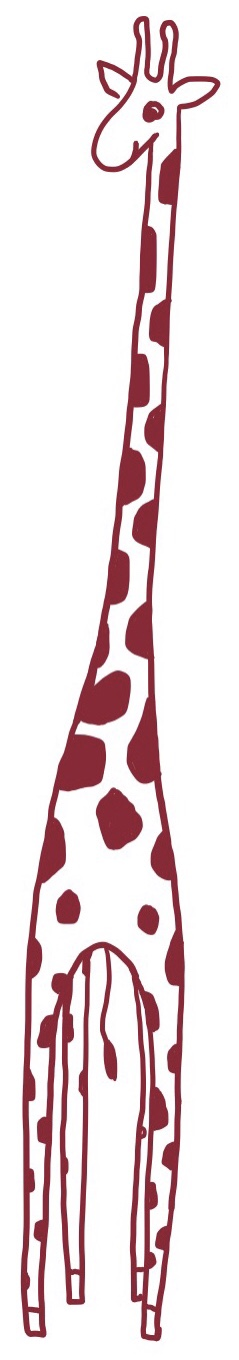
\includegraphics[scale=0.34]{pic/giraff.png}
\end{textblock*}
\begin{textblock*}{\textwidth}(34cm,25.5cm)
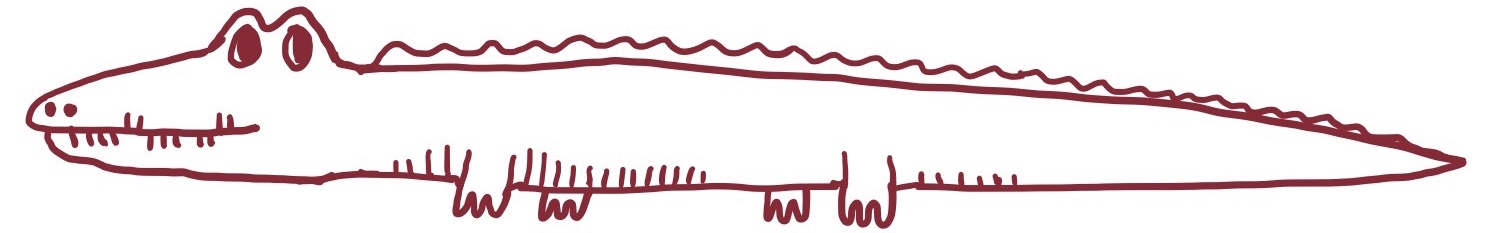
\includegraphics[scale=0.29]{pic/croc.png}
\end{textblock*}
% \begin{textblock*}{\textwidth}(6cm,8cm)
% 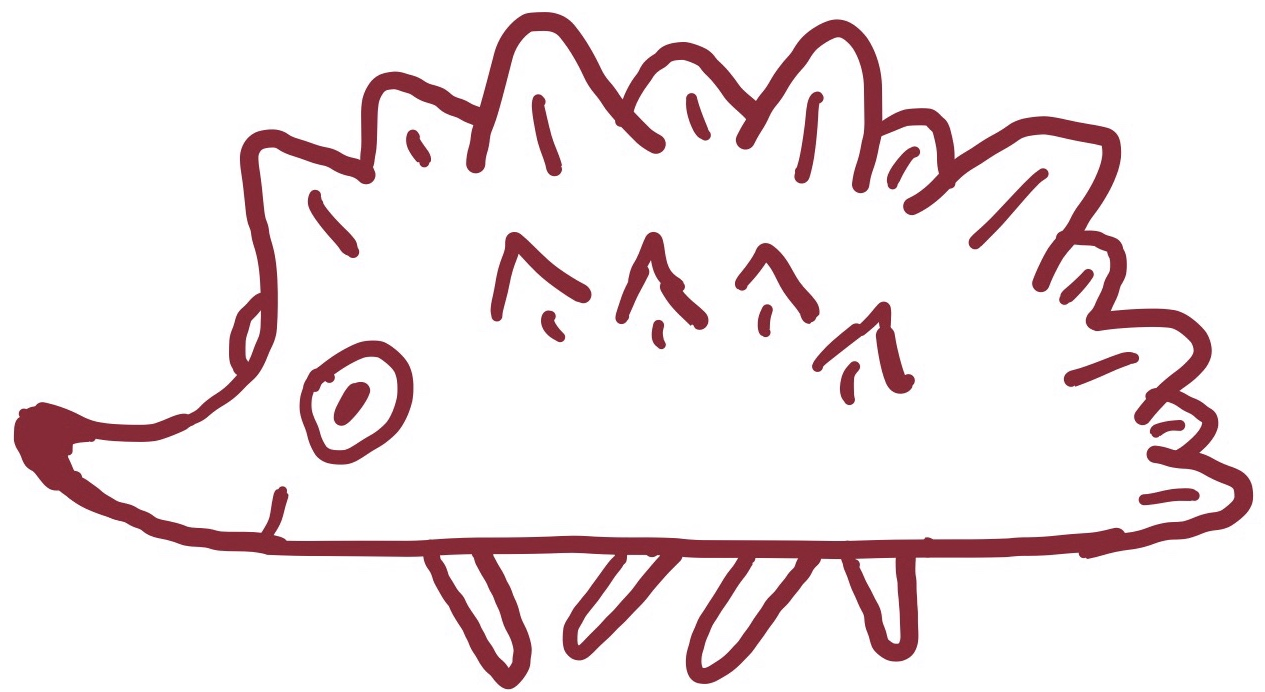
\includegraphics[scale=0.25]{pic/hedge.png}
% \end{textblock*}
%\begin{textblock*}{\textwidth}(10cm,8cm)
%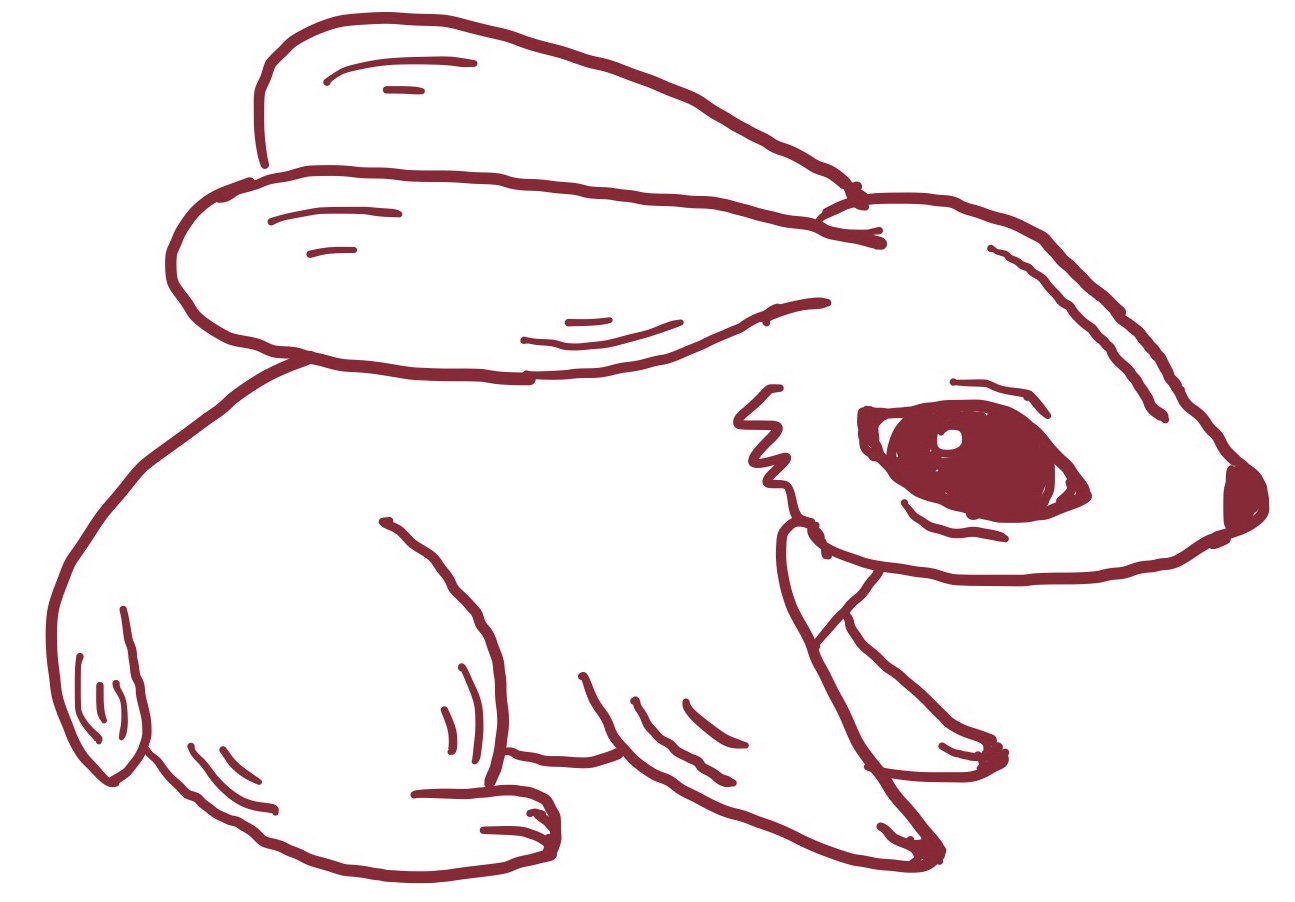
\includegraphics[scale=0.25]{pic/rabbit.png}
%\end{textblock*}
\begin{textblock*}{\textwidth}(32cm,111cm)

\includegraphics[scale=0.40]{pic/snake.png}
\end{textblock*}

\begin{columns}[t]
    \separatorcolumn
    \begin{column}{0.6\paperwidth}
    \begin{block}{Introduction: the Task and the Assessment}
        \textbf{Categorical verbal fluency test} - naming as many items from a semantic category as possible in one minute.
        \vspace{1em}
        \begin{columns}[t]
        \separatorcolumn
        \begin{column}{0.1\paperwidth}
        Widely used in:
        \begin{itemize}
            \item neurology 
            \item psychiatry
            \item clinical linguistics
        \end{itemize}
        \end{column}
        \begin{column}{0.2\paperwidth}
            Methods of scoring:
            \begin{itemize}
                \item traditional: unique words produced
                \item w2v pairwise similarity of adjacent words
                \item clusters produced
            \end{itemize}
        \end{column}
        \begin{column}{0.3\paperwidth}
            Usually, the number of clusters is assessed manually, but it is
           \begin{itemize}
               \item time-consuming
               \item inconsistent (high inter-rater agreement is hard to achieve)
               \item no instruction exists for Russian \cite{drozd2015}
           \end{itemize}
        \end{column}
        \separatorcolumn
        \end{columns}
        \vspace{1em}
        Several methods of automated cluster detection were proposed, most notably \cite{kim2019}. This article is an adaptation of some of the methods used in \cite{kim2019} to the Russian language.
    \end{block}
    \end{column}
    \separatorcolumn
    \begin{column}{0.25\paperwidth}
     \begin{block}{Data}
        46 healthy speakers of Russian (age, gender and education years are all linearly independent)
        \begin{itemize}
           \item ages from 18 to 75 (M = 41.17, SD = 19.53)
           \item 10 to 19 years of education (M = 14.94, SD = 2.54)
           \item 24 females
        \end{itemize}
        46 one category fluency task for the “animal” category transcripts, lemmatized, and the manual clustering by a trained psychiatrist for the transcripts.
    \end{block}
    \end{column}
    \separatorcolumn
\end{columns}

\begin{columns}[t]
\separatorcolumn

\begin{column}{\colwidth}

  \begin{block}{Clustering Methods}
    \begin{itemize}
      \item threshold cutoff:
      \begin{itemize}
          \item at the median (c\_cut\_median)
          \item at the mean (c\_cut\_mean)
          \item at the 25th percentile (c\_cut\_p25)
          \item at the average cosine similarity of each participant (c\_cut\_mean\_local)
      \end{itemize}
      \item sharp change (c\_sharp\_) at difference factors of 0.5, 0.8, 0.95, 1.05, 1.005, and 1.00001. 
    \end{itemize}
  \end{block}

\end{column}

\separatorcolumn

\begin{column}{0.55\paperwidth}

  \begin{block}{Model Selection}
  \begin{itemize}
      \item from models (https://rusvectores.org/ru/models/) scoring the highest  on semantic similarity tasks selected 4 models
      \item assessed number of out-of-vocabulary words (oov, e.g. "трубкозуб")
      \item assessed the range of cosine similarity as a measure of how well-represented animal lexicon is
  \end{itemize}
    Selected the model with the lowest oov and highest range of cosine similarity: tayga\_upos\_skipgram\_300\_2\_2019 with a~5~bn words training set \cite{KutuzovKuzmenko2017}.
  \end{block}
\end{column}
\separatorcolumn
\end{columns}

\begin{columns}[t]
    \separatorcolumn
    \setlength\arrayrulewidth{1pt}

    \begin{column}{0.9\paperwidth}
        \begin{block}{Examples of Clustering by Different Methods}
\begin{table}
\centering
\begin{tabular}{lc|ccccc|ccc|cccc|cc|c|c|ccc|c}
\multicolumn{2}{r}{elephant}                        & hare & wolf                      & deer                       & kangaroo                     & \multicolumn{1}{c}{giraffe} & gopher                      & hamster                      & \multicolumn{1}{c}{rabbit} & penguin                      & ostrich                     & \small{rhinoceros}                   & \multicolumn{1}{c}{crocodile} & brown bear    & \multicolumn{1}{c}{polar bear}    & \multicolumn{1}{c}{panda} & \multicolumn{1}{c}{grizzly} &                         &                         & \multicolumn{1}{c}{kolobok} & boa   \\ 
\hline
 \textbf{correct}        & слон                     & заяц & волк                      & \multicolumn{1}{c|}{олень} & кенгуру                      & жираф                       & суслик                      & хомячок                      & кролик                     & пингвин                      & \multicolumn{1}{c|}{страус} & носорог                      & \multicolumn{1}{c}{крокодил}\multicolumn{1}{c|}  & бурый медведь & \multicolumn{1}{c}{белый медведь} & \multicolumn{1}{c}{панда} & гризли                      & уж                      & \multicolumn{1}{c|}{еж} & колобок                     & удав  \\
\textbf{median}          & \multicolumn{1}{c}{слон} & заяц & волк                      & олень                      & кенгуру                      & жираф                       & суслик                      & хомячок                      & кролик                     & пингвин                      & страус                      & носорог                      & крокодил                      & бурый медведь & белый медведь                     & панда                     & гризли                      & \multicolumn{1}{c|}{уж} & \multicolumn{1}{c|}{еж} & колобок                     & удав  \\
 \textbf{local mean}     & слон                     & заяц & волк                      & олень                      & кенгуру                      & жираф                       & суслик                      & хомячок                      & \multicolumn{1}{c}{кролик} & пингвин                      & страус                      & носорог                      & крокодил                      & бурый медведь & белый медведь                     & панда                     & гризли                      & \multicolumn{1}{c|}{уж} & \multicolumn{1}{c|}{еж} & колобок                     & удав  \\
\textbf{sharp 0.8}       & слон                     & заяц & \multicolumn{1}{c|}{волк} & \multicolumn{1}{c|}{олень} & \multicolumn{1}{c|}{кенгуру} & жираф                       & \multicolumn{1}{c|}{суслик} & \multicolumn{1}{c|}{хомячок} & кролик                     & \multicolumn{1}{c|}{пингвин} & \multicolumn{1}{c|}{страус} & \multicolumn{1}{c|}{носорог} & крокодил                      & бурый медведь & белый медведь                     & панда                     & гризли                      & уж                      & еж                      & колобок                     & удав  \\
 \textbf{sharp 1.00001}~ & \multicolumn{1}{c}{слон} & заяц & волк                      & \multicolumn{1}{c|}{олень} & кенгуру                      & жираф                       & суслик                      & хомячок                      & кролик                     & пингвин                      & страус                      & носорог                      & крокодил                      & бурый медведь & белый медведь                     & панда                     & гризли                      & уж                      & еж                      & колобок                     & удав 
\end{tabular}
\end{table}
        \end{block}
    \end{column}
    \separatorcolumn
\end{columns}

\begin{columns}[t]
    \separatorcolumn
    \begin{column}{0.2\paperwidth}
        \begin{block}{Number of clusters and Age}
            In theory \cite{kim2019} older people produce fewer clusters And we also have the same result: p  ≈  0.01 (p<0.05), r  ≈  -0.37.
    
            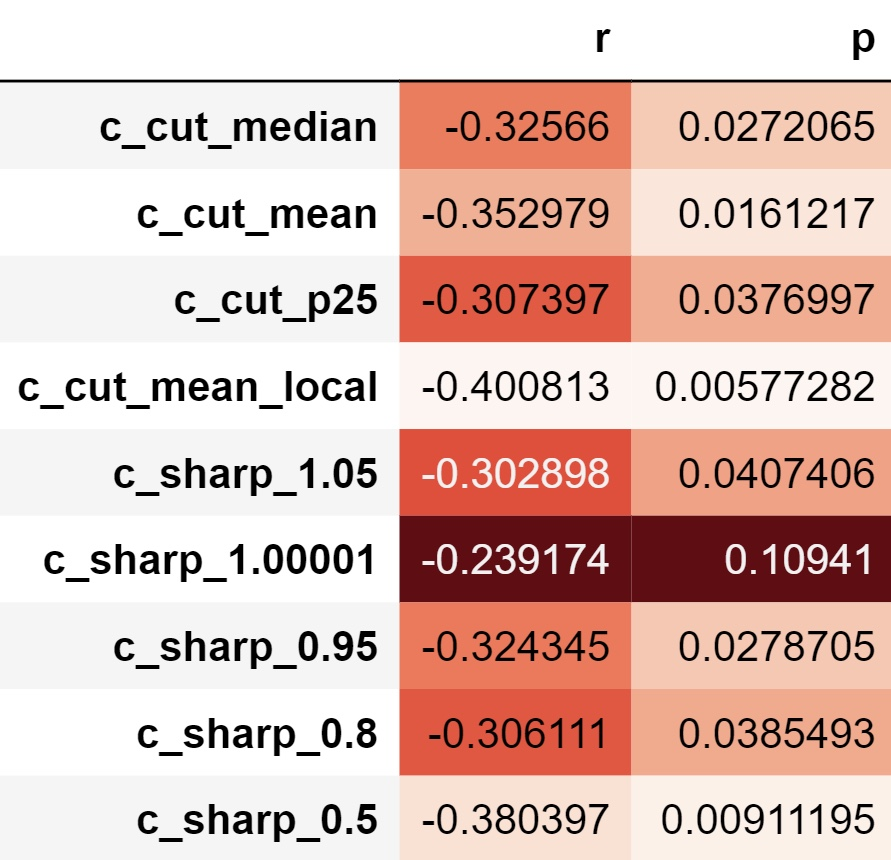
\includegraphics[scale=0.9]{pic/correlation_with_age.png}
        
             All, but sharp change at 0.00001, do correlate negatively with age, the strongest being \alert{cutoff at the local mean} (r  ≈  -0.4, p  ≈  0.006), \alert{sharp change at 0.5} (r  ≈  -0.38, p  ≈  0.009), alert{cutoff at the mean} (r  ≈  -0.35, p  ≈  0.01).
             
             Metrics of cutting at the local mean and sharp change at 0.5 are more strongly correlated with age than manual splits.
             
             Nothing else is correlated (number of splits by any metric with education years or gender, age or education years with oov or average cosine similarity - but we did not expect it to)
        \end{block}
    \end{column}
    \separatorcolumn
    \begin{column}{0.2\paperwidth}
        \begin{block}{Manual scoring}
            Spearman's correlation of manually calculated number of clusters with different approximations methods.
            
            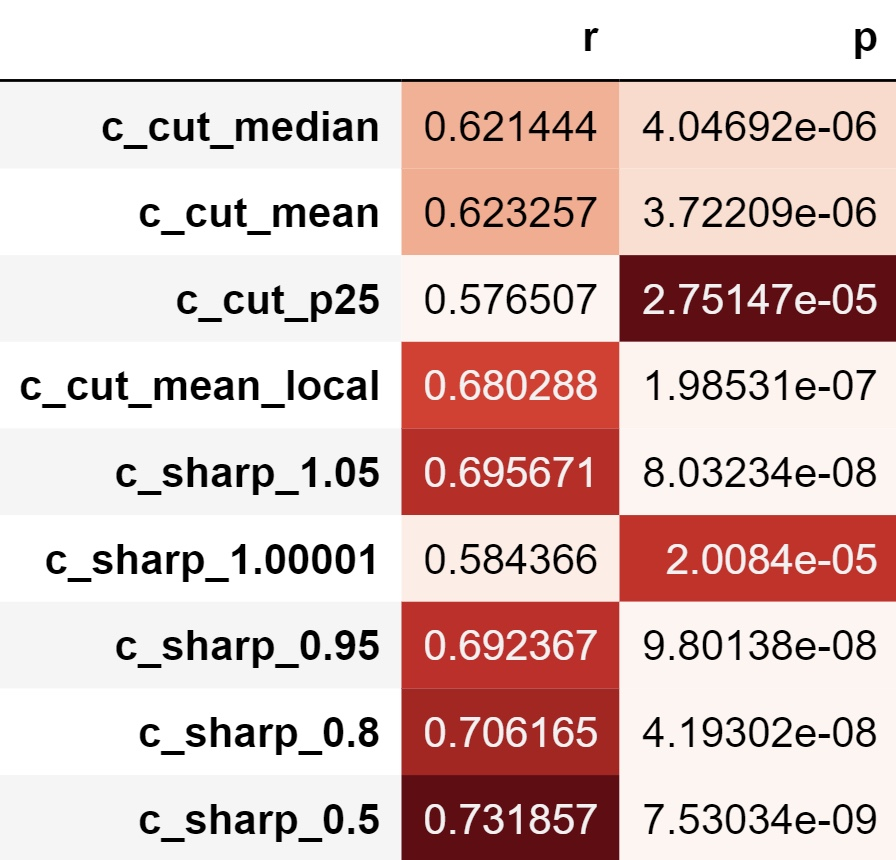
\includegraphics[scale=0.9]{pic/correlation_with_correct_scoring.png}
            
            All methods of getting the number of splits are good enough at approximating manual calculation, the best being \alert{sharp change metrics with factors 0.5, 0.8}, 0.95, 1.05 (r ≈ 0.73 for 0.5, r ≈ 0.7 for others) and \alert{cutoff at the local mean} (r ≈ 0.7).
            
            However, the factors of 0.5 and 0.8 produce on average too many splits (16 and 12), and the best at approximating not the ranks but the actual numbers (10 clusters on average) are probably the ones with approximately 9  clusters - \alert{sharp change metrics at 1.05 and 0.95} and \alert{cutoff at the local mean}.
        \end{block}
    \end{column}
    \separatorcolumn
    \begin{column}{0.4\paperwidth}
        \begin{block}{Quality of Cluster Boundary Positioning}
            Here we use accuracy, precision, recall, f1-measure and weighted f-measure to determine the quality of cluster boundaries positioning. For the task at hand precision is more important than recall.
            
            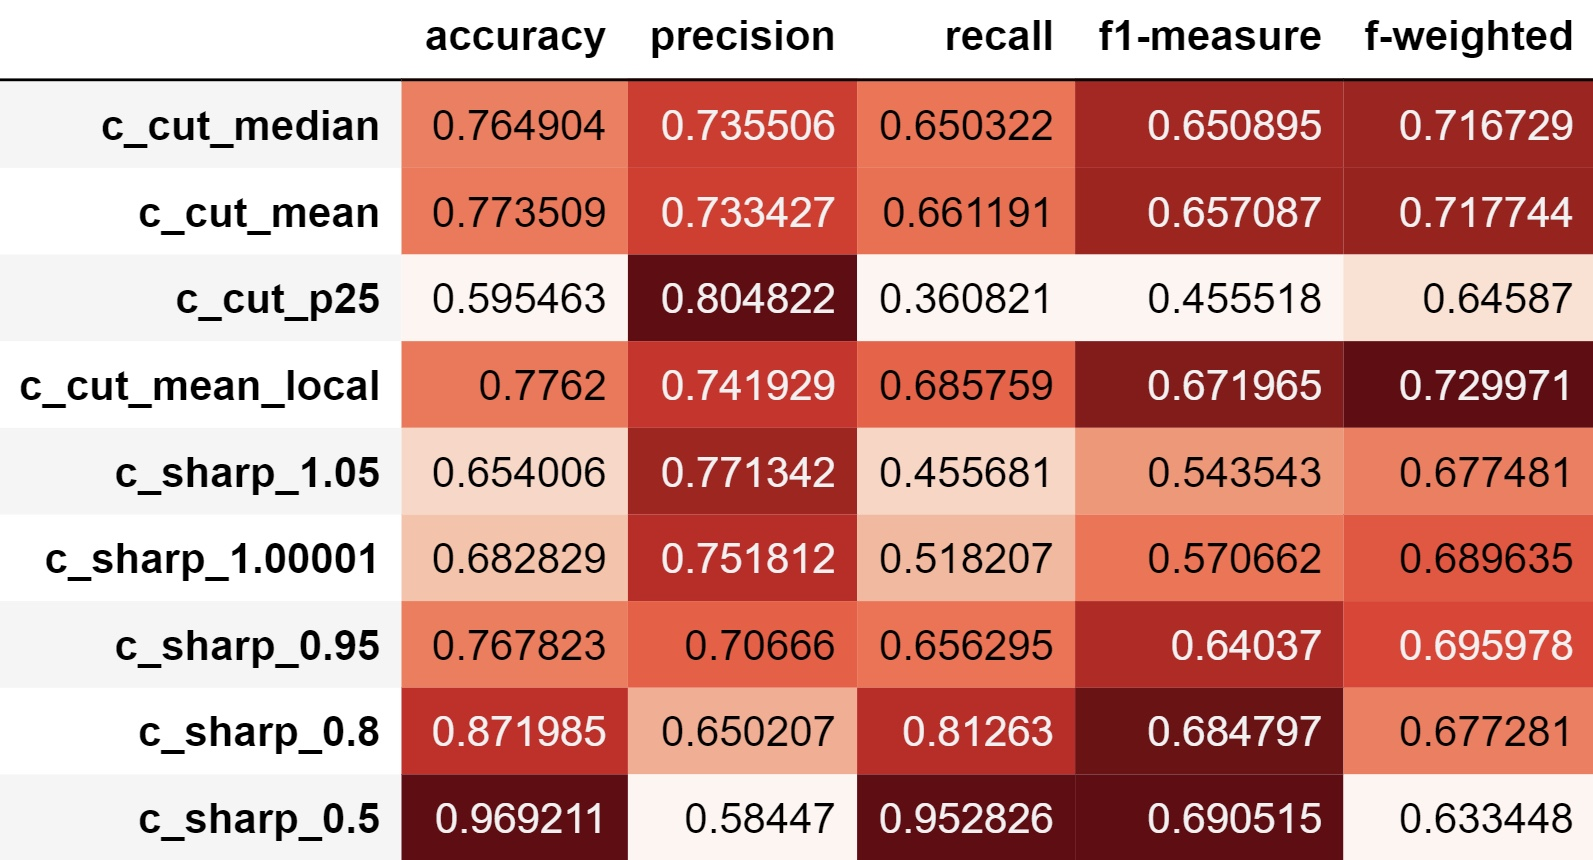
\includegraphics[scale=0.9]{pic/metrics_of_positioning_table.png}
            
            \alert{Cutoff at the mean} is the best at catching all correct values (but poor at not-catching incorrect splits - making too many splits).
            
            \alert{Sharp change metrics at 1.05 to 0.95} are good at only catching correct values (but bad at identifying all splits - making too little splits)
            
            As we care more about only identifying correct splits (precision), then on identifying all correct splits (recall), we use 0.5 weighted f-measure
            
            $${\displaystyle F_{\beta }=(1+\beta ^{2})\cdot {\frac {\mathrm {precision} \cdot \mathrm {recall} }{\beta ^{2}\cdot \mathrm {precision} +\mathrm {recall} }}}$$
            
            The best metrics by weighed f-measure are: \alert{cutoff at the local mean}, sharp change metrics (1.05 to 0.95), and cutoff at the mean.  Overall the metrics are good-ish (0.7 is not all that good but tolerable).
        \end{block}
    \end{column}
    \separatorcolumn
\end{columns}
\begin{columns}[t]
    \begin{column}{0.3\paperwidth}
        \begin{block}{Results}
        This work successfully adapts some of the methods used in \cite{kim2019} to Russian language. It proves it is possible to automatically approximate both number of clusters and their positioning. For the given model the best metrics across the tasks are:
        
        \begin{itemize}
            \item cutoff at the local mean, that was proposed, but not realized in \cite{kim2019}
            \item sharp change  measure with the factor of 0.95
            \item cutoff at the mean or median of the whole dataset
        \end{itemize}
        \end{block}
    \end{column}
    \begin{column}{0.55\paperwidth}
        \begin{block}{Future Research}
        The results might be improved by:
        \begin{itemize}
            \item using several raters to tag manual clustering (although high inter-rater agreement might be hard to achieve)
            \item tagging non-semantic associations as separate clusters, as "утка-лебедь-рак-щука" would be tagged one under current manual clustering
            \item solving out-of-vocabulary issues and poor representation of animal lexicon by using transfer learning (additionally training the model for the specific category) 
            \item assessing the convexity of the curves of change in the number of clusters as one lowers the threshold
            \item comparing more of the models that are available for Russian language
        \end{itemize}
        \end{block}
    \end{column}
\end{columns}
\begin{columns}
    \separatorcolumn
    \begin{column}{0.9\paperwidth}
        \begin{block}{~}
            \heading{References}
            \nocite*
            \bibliographystyle{apalike}\bibliography{poster}
        \end{block}
    \end{column}
    \separatorcolumn
\end{columns}

\end{frame}



\end{document}
